The \textbf{SpiNNaker} system is a massively-parallel, bio-inspired computing platform. The goal of the project is to build a machine that will contain $\sim$1 million CPU cores and will be able to simulate $\sim$1 billion neurons in real time. As any multi-core system, communication between cores is basic; the SpiNNaker chip has been designed to efficiently implement neural networks, thus, networking is specialized (but not limited) to transmit spikes. There are currently two board models the Spinn-3, which hosts 4 SpiNNaker chips, and the Spinn-4 that houses 48 nodes. These boards are also known as 102 and 103 machines, respectively. Larger systems will be built using Spinn-4 boards as the basic construction block. Plans include building the following: 
\begin{description}
  \item[104 machine], a 12 Spinn-4 desktop frame with $\sim$10000 ARM cores.
  \item[105 machine], five card frames with 24 Spinn-4 each allocated in a rack cabinet ($\sim$100,000 cores).
  \item[106 machine], 10 racks, each with similar capacities of the 105 machine ($\sim$1,000,000 cores).
\end{description}

\subsection{SpiNNaker chip overview}

SpiNNaker chips consist of 18 ARM968 cores, each with tightly-coupled program and data memory. Each core also has a Communication Network-on-Chip (C-NoC) interface that, with the help of an in-die network router, allows inter- and intra-chip communications (Figure~\ref{fig:hw:spinnaker-die}). On top of the chip lie 128 MBytes of Synchronous Dynamic RAM (SDRAM) whose die is stitch-bonded to the chip for faster access (Figure~\ref{fig:hw:bonded-sdram}). The SpiNNaker chip plus the SDRAM are sometimes referred as a \emph{node}~\cite{furber2013overview}.

\begin{figure}[h]
  \begin{center}
    \begin{subfigure}[b]{0.55\textwidth}
      \includegraphics[width=\textwidth]{spinn_labeled_bw}
      \caption{SpiNNaker chip die.}
      \label{fig:hw:spinnaker-die}
    \end{subfigure}
    \hspace*{0.3cm}
    \begin{subfigure}[b]{0.4\textwidth}
      \includegraphics[width=\textwidth]{spinn_dies-ram}
      \caption{Stitch-bonded SDRAM on top of the SpiNNaker chip.}
      \label{fig:hw:bonded-sdram}
    \end{subfigure}
    \caption{SpiNNaker base component, a node, consists of a multi-core chip with stitch-bonded SDRAM.}
  \end{center}
\end{figure}

One of the cores acts as a system controller and, typically, 16 cores will run the applications. Any processor in a chip will have access to four memory spaces. Instruction and data memories are only locally visible (i.e. a core can only see its local memory). These two spaces are composed of a 32 and 64 KByte tightly-coupled blocks of memory, respectively. There are also a 32 KByte block of on-chip SRAM and the 128 MByte off-die SDRAM, both of them are node-local (i.e. seen by all processors in the chip). The cores are able to access the SDRAM and SRAM using the System Network-on-Chip (S-NoC) and no inter-chip memory coherence mechanisms are present~\cite{furber2013overview}. SDRAM is commonly used for large data structures like synaptic weight matrices, while the SRAM is used for core-to-core message passing.

\subsection{Communications}

One of the notable aspects of the SpiNNaker system is the flexibility of its networking infrastructure. Communication in the global scale is asynchronous and locally synchronous. There are six direct links from any source node to its neighbours. This provides sufficient connections to form an efficient network that may be configured to form a toroid (Figure~\ref{fig:hw:spinn-toroid}) on a 2D circuit board.

\begin{figure}[h]
  \begin{center}
    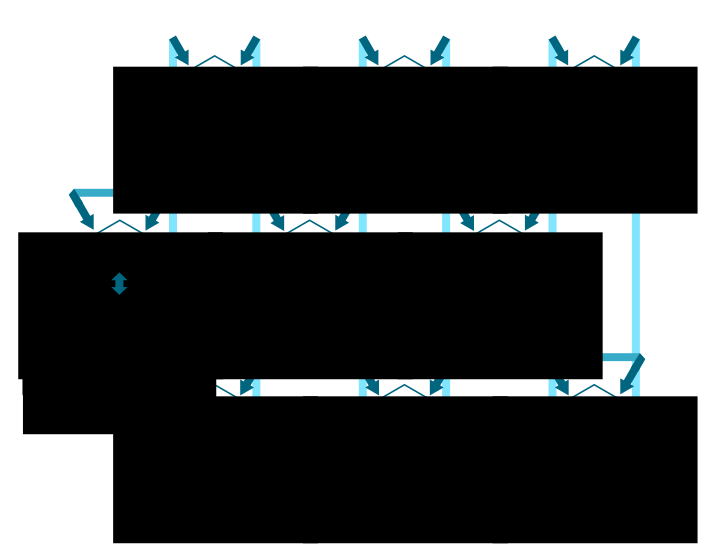
\includegraphics[width=0.7\textwidth]{spinn-interconect}
    \caption{Nine SpiNNaker nodes connected as a toroid.}
    \label{fig:hw:spinn-toroid}
  \end{center}
\end{figure}

Packets are the only way a SpiNNaker chip can communicate to another; a core sends a packet to the local router where it's forwarded to one or more targets. If the target is in the same node, the router will deliver it directly; otherwise, the router sends the packet to an adjacent node where the next router will decide the appropriate move. Packets are either 40 or 72 bit long, a control byte, and one or two 32-bit words.

There are four ways a packet types, each of which are routed differently by the router. \emph{Nearest neighbour} (NN) and \emph{point-to-point} (P2P) packets are may be generated by any core, but will only reach the monitor core on the target node. NN packets are mainly used for boot and recovery and P2P for code distribution and system control. \emph{Fixed route} (FR) packets may be emitted by any core and sent to any other core, though the route is may not be changed once an application is running. This packet type is generally used for debugging purposes.
The \emph{multicast} (MC) packet also permits core-to-core transmission, so applications use this type to transmit data. If the packet has multiple targets, a router along the way will duplicate it and fork the route. This is a highly desired feature for neural applications, since one neuron's axon may connect to multiple neurons dendrites~\cite{spinn-net-patterson2012scalable}. MC packets are formed using address event representation (AER), so they posses a time-stamp and a full source address (node, core, and neuron identifications).

Communication to the outside world is done through 100 Mbit/s Ethernet, General Purpose Input/Output (GPIO) lines and through Field-Programmable Gate Arrays (FPGAs, on the 48-node boards).

\subsection{Programming modes}
Since neurons are thought to react as spikes arrive at their dendrites, SpiNNaker chips support event-based usage via specialized interrupt hardware. There are, primarily, two choices while trying to program SpiNNaker. 

The first is through the application programming interface (API) following an event-driven model. In this way applications can only specify what functions to execute when an event occurred. Events include multicast packet reception, direct memory access (DMA) completion, timer ticks, SpiNNaker datagram protocol packet arrival, and custom user events. Using this type of programming allows developers to create not only neural network simulations but any application~\cite{spinn-software-docs}. 

The second is to use the neural network interface PyNN~\cite{davison2008pynn}, which provides a common front-end to different simulators (e.g. NEST, Brian, sPyNNaker). Since the descriptions are stated using the Python programming language and because it's a high level description, the learning curve for this approach is moderate~\cite{spynnaker-github}. A common PyNN application would set-up the simulator parameters, describe neural populations, establish the appropriate projections and start the simulation. The sPyNNaker team has added modules for real-time interaction with PyNN scripts and facilities for adding new neural and synaptic models.